\section{Assvengers}

El presidente ha citado a los "assvengers" a un consejo de héroes latinoamericanos, con el fin de  definir lo que van a hacer contra un Hulk naranjado que quiere ponerle aranceles  a toda latinoamérica. La reunión  iba bien hasta que los héroes se lo tomaron personal, lloraron y alegaron, ya que todos estaban en desacuerdo con la decisión del presidente  de incluir  al Lagarto  en su consejo.

\subsection{Procedimiento gráfico (1.3 pt)}

El primero en quejarse fue el Capitán Sur América ya que el lagarto no cree que el nuevo Capitán  sea tan "papucho" como el anterior y lo tiene mal condicionado. Si la función de inestabilidad psicológica del Capi es:

\[ f(x) = \ln{x} + \frac{1}{x-c} \]
\[ f(x) = \ln{x} + \frac{1}{x-0} \]
\[ g(x) = \left|\frac{xf'(x)}{f(x)}\right| \]
\[ Z(x) = 1 \]

\begin{figure}[H]
    \centering
    \begin{subfigure}[b]{\textwidth}
        \centering
        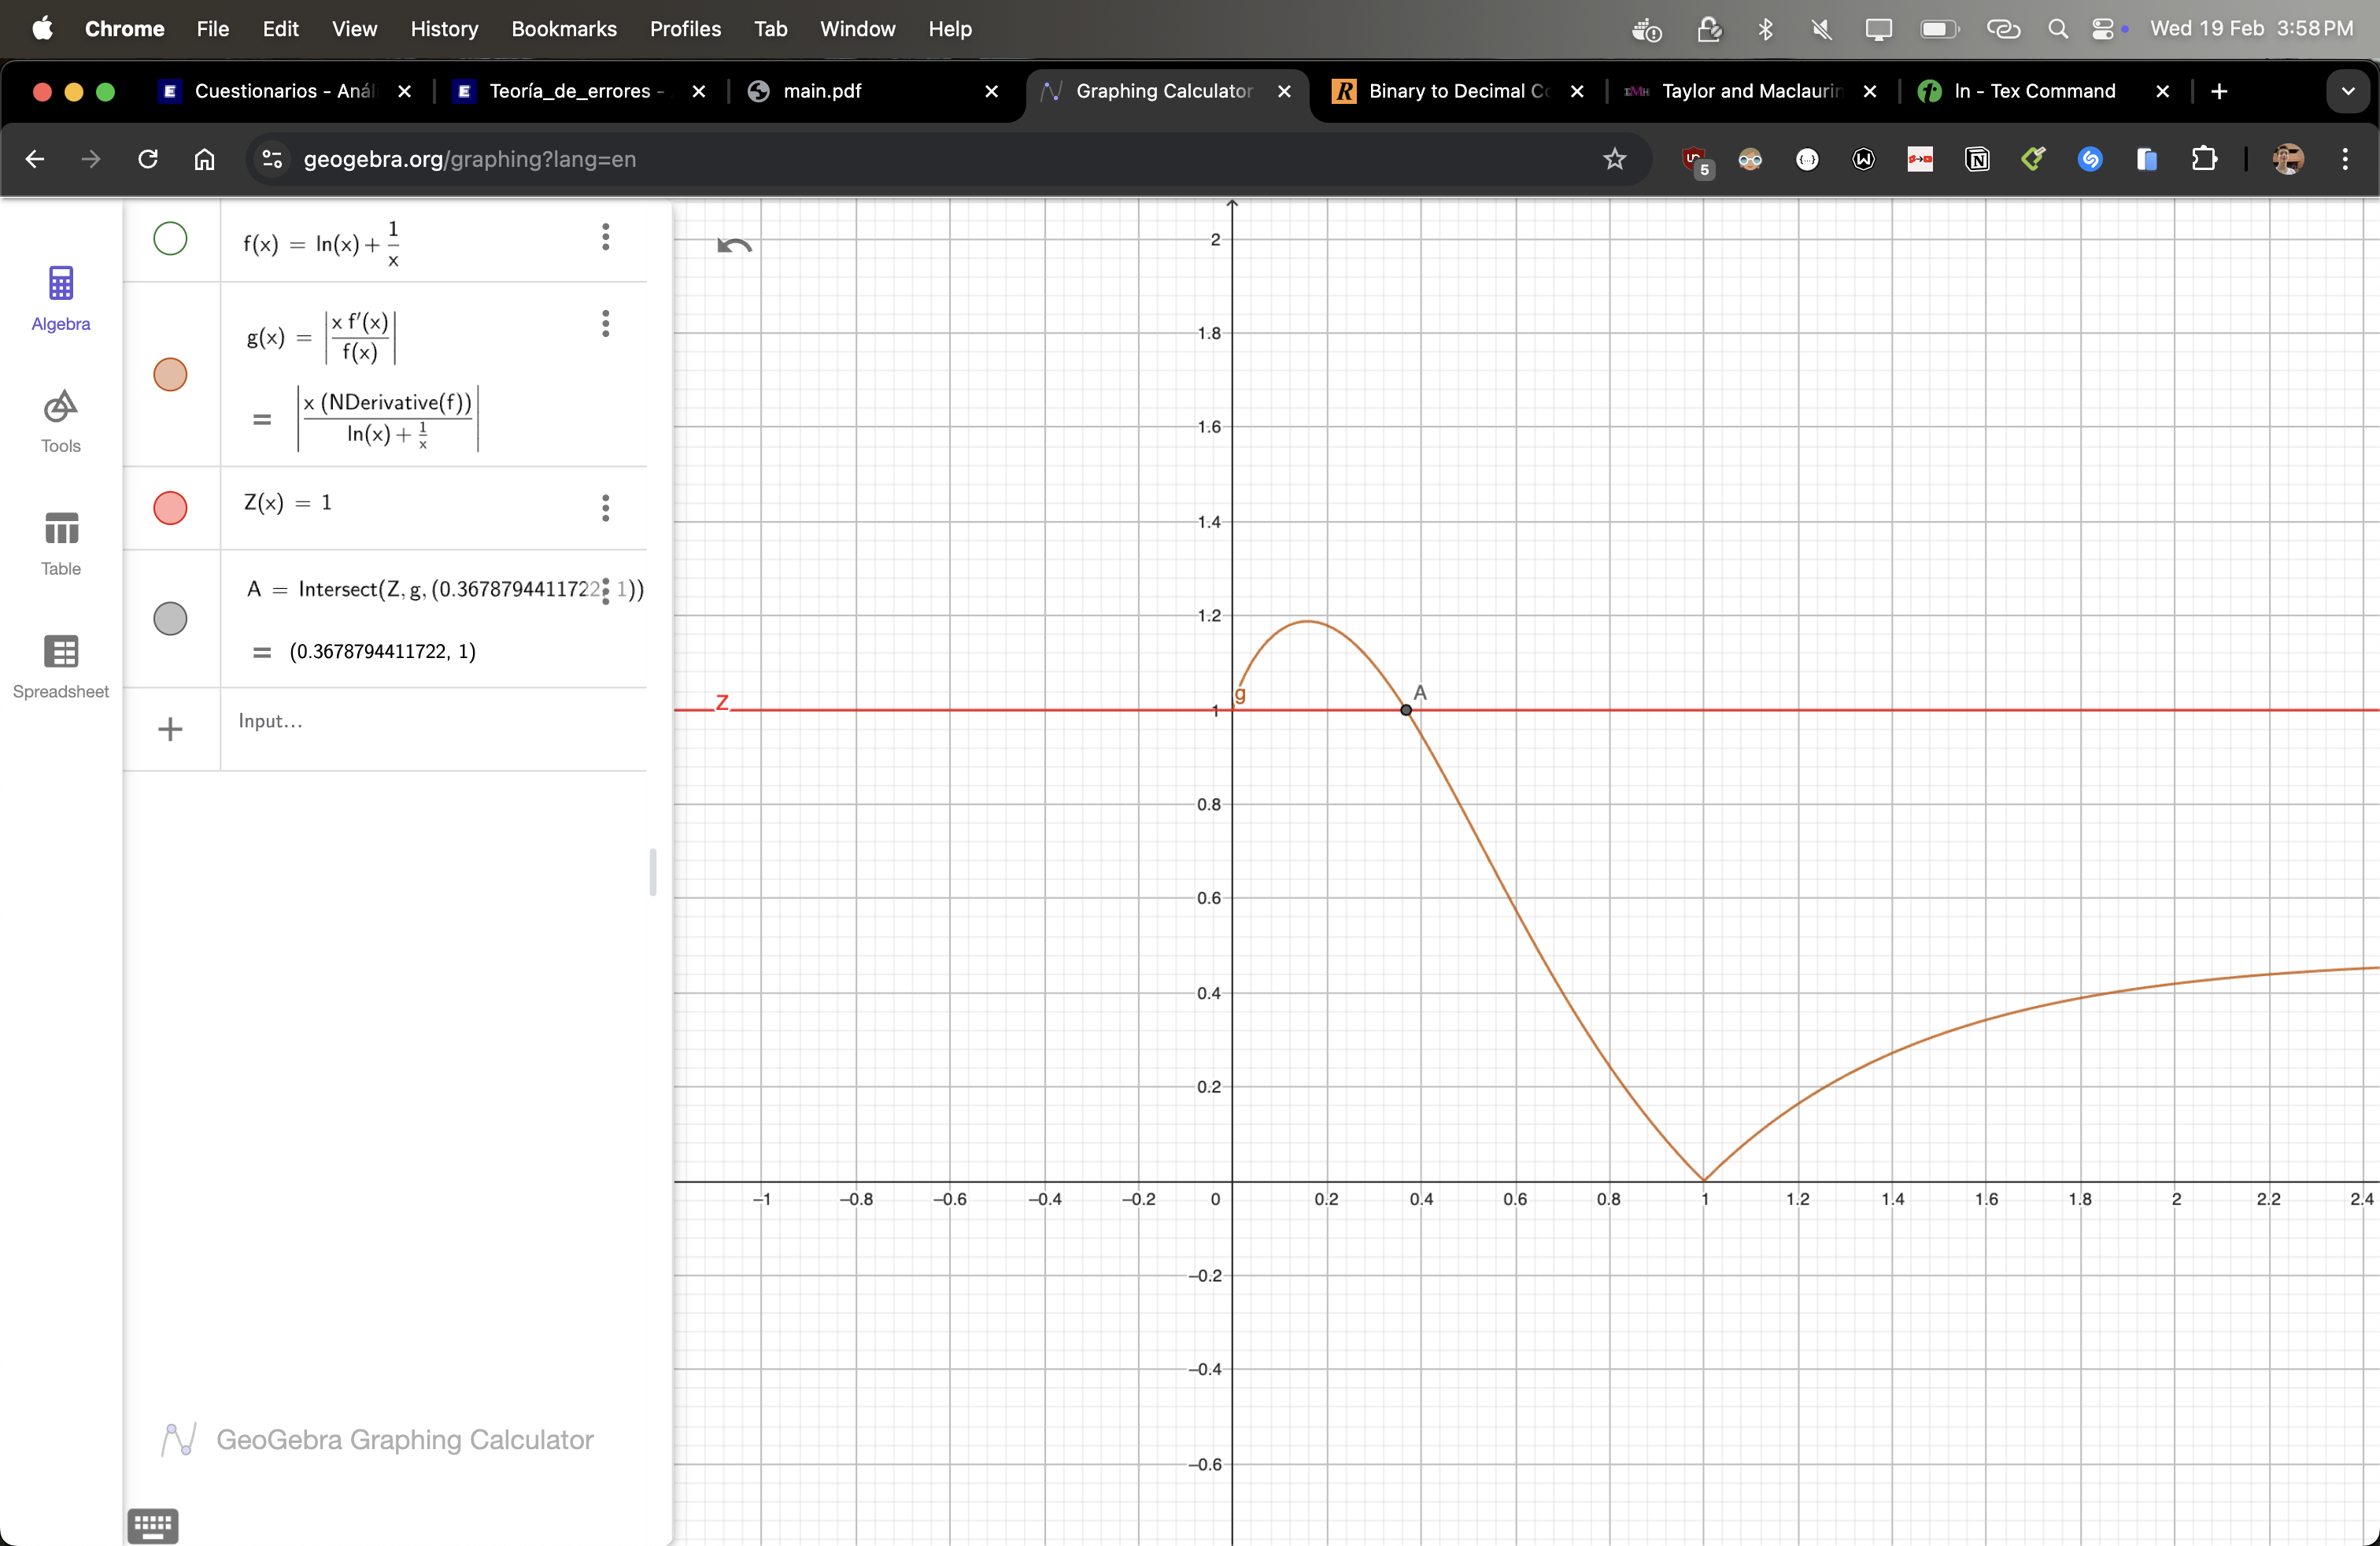
\includegraphics[width=\textwidth]{Figures/0. General/1.1.png}
        \caption{Gráfica g(x) con el intersecto sobre Z(x)}
        \label{fig: Grafica g(x)}
    \end{subfigure}
\end{figure}

De $0$ a el Intersecto $A$ $(0.368, 1)$ la función $g(x)$ (en este caso la función de condición)
es mayor que 1, y de $0.368$ a $\infty$ la función $g(x)$ es menor que 1. Por lo tanto,
la inestabilidad de Capitán Sur América está mal condicionada en el intervalo $[0, 0.368]$.

\subsection{Aproximación de Taylor (1.3 pt)}
El número de condición anterior también representa el mal condicionamiento de toda latinoamérica, y sirve para encontrar los aranceles que nos va a imponer el Hulk naranja, sin embargo, es necesario usar una aproximación de Taylor  de tres términos centrada en 2 para el número de condición . Encuentre la aproximación de Taylor que representa los aranceles.


\subsection{Exactitud (1.4 pt)}

Otro momento importante  de la reunión  fue cuando "Novelaman" le confesó al presidente  su amor y decidió  pagar los aranceles anteriores como regalo de San Valentín. En principio él necesita saber cuánto representan estos aranceles cuando la aproximación de Taylor se evalúa en dos de los valores del intervalo de mal condicionamiento (ejercicio 1). Para estar seguro que no lo están robando, Novelaman calcula también los aranceles con el número de condición verdadero, pero no obtiene los mismos resultados, así que afirma que el Lagarto se está robando la platica.  Calcule usted las exactitudes que tienen dos valores pertenecientes al intervalo de mal condicionamiento del ejercicio 1 y explique a Novelaman, porque le dan diferentes las exactitudes.  (Puede usar cualquier valor de su elección en el intervalo de mal condicionamieto) Entregue su procedimiento y explicación.